% ============================================================
% Chapter 1 — Overview: Prototypes, Products & the Business of Engineering
% Folder: chapters/01-overview
% ============================================================

\chapter{Overview: Prototypes, Products \& the Business of Engineering}
\label{ch:overview}

Every project begins with a claim: \emph{this idea is worth building.}
Your job in Project~I is to find out whether that claim is true---cheaply,
quickly, and with enough documentation that the answer is defensible.
By the end of this course you will have built a working proof-of-concept,
assembled the record that shows how you got there, and produced the
business case that connects your hands-on work to the real world of
engineering firms and markets.
This chapter gives you the map.
You will see what you are building, why it matters, what separates a
prototype from a finished product, and what turns a validated prototype
into revenue.

% ──────────────────────────────────────────────────────────
\section*{Learning Objectives}
% ──────────────────────────────────────────────────────────
\begin{enumerate}
  \item State what a prototype is for and describe the two deliverables
        you will produce in Project~I.
  \item Describe how a proven prototype becomes a product and identify
        the link between Project~I and Project~II.
  \item Explain your role as a technician working alongside engineers.
  \item Explain why industry work is justified by the value it creates,
        and interpret a negative economic finding correctly.
  \item Identify the principal business models that turn a validated
        prototype into revenue.
\end{enumerate}

% ──────────────────────────────────────────────────────────
\section{What You Will Build}
\label{sec:ch1-what-you-build}
% ──────────────────────────────────────────────────────────

You will build two things: a \textbf{proof-of-concept prototype} and
\textbf{the record of how you got there.}
\index{proof-of-concept}

The prototype is a working artifact that answers a specific technical and
business question.
It does not need to be pretty, manufacturable, or certifiable.
It needs to demonstrate that the core idea functions under realistic
conditions.

The record is a portfolio of documents---specification, risk register,
architecture diagrams, build logs, test data, and cost analysis---that
accumulate as you work.
You do not write the portfolio at the end.
You assemble it from artifacts you produce at each stage.
If you work that way, the portfolio is nearly complete before you realize
you are making one.

Together, the prototype and its record constitute your output from Project~I.
The record is as important as the hardware: an engineer can reproduce,
evaluate, and extend documented work; undocumented work is disposable.

% ──────────────────────────────────────────────────────────
\section{The Course Map: Two Tracks Over Twelve Weeks}
\label{sec:ch1-course-map}
% ──────────────────────────────────────────────────────────

Figure~\ref{fig:ch1-pipeline} shows the full engineering journey from
concept to market.
Project~I occupies the second stage---the prototype---and Project~II the
third, where the proven concept is developed into a manufacturable product.
The arrow between them is not automatic: what crosses it is the
documentation you create in Project~I.

\begin{figure}[htbp]
  \centering
  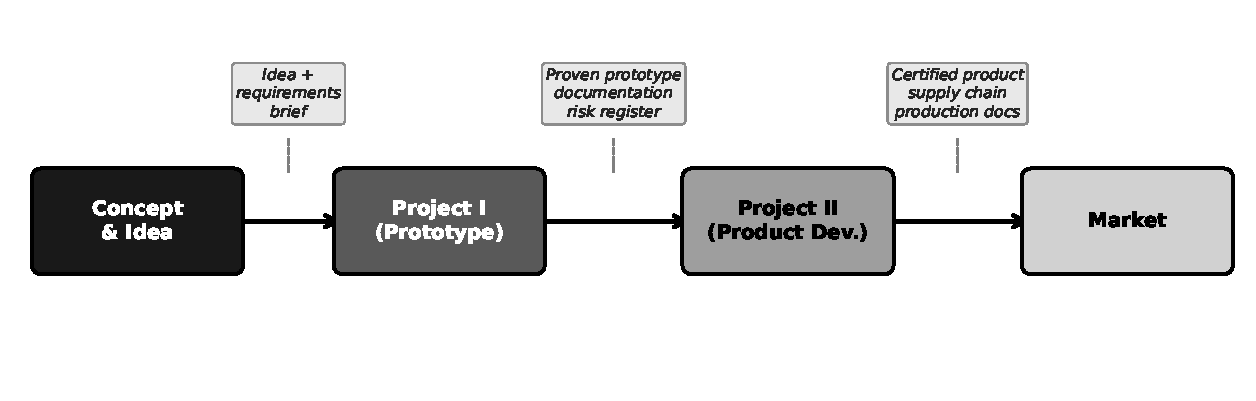
\includegraphics[width=0.85\textwidth]{images/fig_01_pipeline.pdf}
  \caption{The engineering pipeline from concept to market.
           Project~I delivers the proven prototype and its documentation;
           Project~II turns that foundation into a manufacturable product.}
  \label{fig:ch1-pipeline}
\end{figure}

The course runs two \textbf{parallel tracks}: a theory track and a lab
(practice) track.
Figure~\ref{fig:ch1-coursemap} shows how they align across the twelve weeks.
\index{theory track}\index{lab track}

\begin{figure}[htbp]
  \centering
  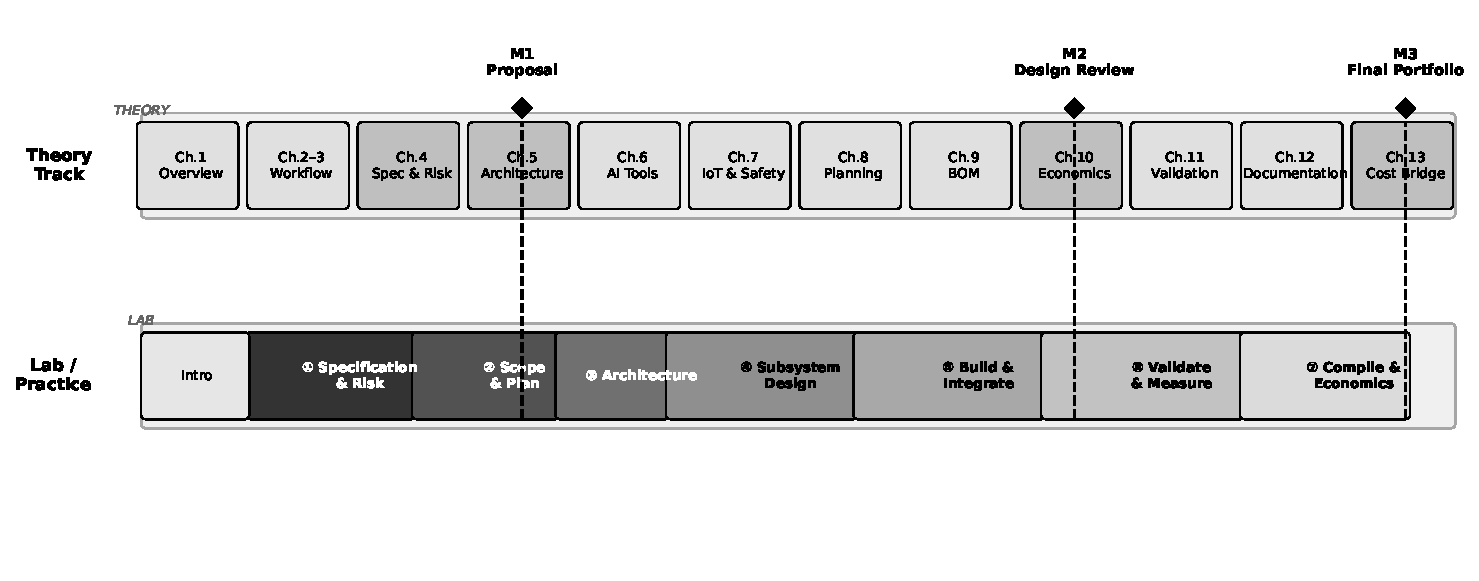
\includegraphics[width=0.85\textwidth]{images/fig_02_course_map.pdf}
  \caption{The two-track course structure over twelve weeks.
           The theory track introduces each topic just before the lab
           requires it; the seven workflow stages unfold across the practice
           track, with three graded milestones (M1–M3).}
  \label{fig:ch1-coursemap}
\end{figure}

The theory track moves through the seventeen chapters of this book at
roughly one to two chapters per week, with Chapter~1 and Chapter~2 paired in Week~1.
The lab track runs the \textbf{seven-stage Prototype Development Cycle},
\index{seven-stage workflow}
which you will study in depth in Chapter~3.
At the overview level, the seven stages are:

\begin{enumerate}
  \item \textbf{Specification \& Risk} --- translate the idea into
        measurable requirements and a risk ranking.
  \item \textbf{Scoping \& Planning} --- decide what you will build,
        set a schedule, and identify long-lead procurement.
  \item \textbf{Architecture} --- decompose the system into subsystems
        and define their interfaces.
  \item \textbf{Subsystem Design} --- make detailed design decisions
        for each subsystem.
  \item \textbf{Build \& Integration} --- fabricate and assemble; bring
        subsystems together.
  \item \textbf{Validate \& Measure} --- test against the specification;
        collect data; decide whether to iterate.
  \item \textbf{Compile \& Economics} --- assemble the portfolio and
        analyse the cost and business case.
\end{enumerate}

Three milestones punctuate the semester.
\textbf{Milestone~1} (Proposal, end of Week~3) delivers your specification
and risk register.
\textbf{Milestone~2} (Design Review, end of Week~9) delivers your
architecture, build records, and preliminary cost analysis.
\textbf{Milestone~3} (Final Portfolio, end of Week~12) delivers the
complete project record.
\index{milestone}

The theory topics are sequenced so that each week's reading lands just
as the lab needs it: you study specifications in Week~3, then immediately
write your own in the lab.
This is not a coincidence---it is the design of the course.

% ──────────────────────────────────────────────────────────
\section{From Prototype to Product: The Gap}
\label{sec:ch1-proto-to-product}
% ──────────────────────────────────────────────────────────

A prototype and a product solve different problems.
A \textbf{prototype}\index{prototype} answers a question about technical
feasibility and business viability.
A \textbf{product}\index{product} is an artifact designed to be made
reliably, in volume, at a cost that leaves margin, by people who were not
involved in the original design, and supported over a service life that
may span years.

The gap between them is real and wide.
A successful prototype does not automatically become a product.
The following properties must be designed in---not bolted on afterward:

\begin{description}
  \item[Manufacturability.] Can the design be made in volume using
        available processes, tooling, and supply chains?
        Hand-soldered one-of-a-kind assemblies are not manufacturable
        at scale.

  \item[Reliability.] Does the design meet a minimum operating life
        under realistic field conditions?
        A prototype that runs for an hour in a lab may fail within a
        week in the field due to thermal cycling, vibration, or humidity.

  \item[Cost at volume.] Is the per-unit cost, at the production volumes
        the business requires, low enough to leave an acceptable margin?
        Chapter~10 develops the cost model in full.

  \item[Certification.] Does the design meet applicable electrical
        safety, radio emissions, and (for IoT and robotics) functional
        safety standards?
        Certification is a legal prerequisite in most markets, not an
        optional finishing step.

  \item[Supportability.] Can the product be diagnosed and repaired by
        field technicians?
        Are replacement parts available over the product lifetime?
        Is the documentation sufficient for a technician who was not
        present at the original build?
\end{description}

None of these properties is addressed in Project~I.
That is not a failure; it is appropriate scope management.
Your job in Project~I is to answer the central technical and business
question as quickly and cheaply as possible.
Project~II then takes that answer as its starting point and builds the
full product around it.
What crosses the boundary is your documentation: the specification,
the architecture, the risk register, the validated design decisions.
The formal process by which a prototype earns the right to become a product --- Stage-Gate --- is introduced in Chapter~2.

\paragraph{In Practice.}
A team building a wearable health monitor completes a functional prototype
in twelve weeks: it reads heart rate, displays data on a small screen, and
transmits to a phone app.
The team is pleased---and surprised, six months later, to learn that the
product redesign for manufacturing took an additional eighteen months.
The enclosure needed injection-moulding tooling.
The radio module required FCC and IC certification.
The battery management circuit had to be redesigned for the thermal
envelope of a wearable.
The prototype proved the concept; the product required a separate,
larger effort.
Neither effort was wasted.

% ──────────────────────────────────────────────────────────
\section{Working with Engineers: What You Own}
\label{sec:ch1-working-with-engineers}
% ──────────────────────────────────────────────────────────

In industry you will work on a team that includes engineers.
Understanding who owns what prevents frustration and makes you more
effective.

\textbf{Engineers}\index{engineer} own:
\begin{itemize}
  \item Requirements---what the system must do, expressed as measurable
        criteria.
  \item Design accountability---the engineer signs off on the architecture
        and carries legal responsibility for the design.
  \item Risk decisions---the call to proceed, stop, or redesign rests
        with the engineer of record.
\end{itemize}

\textbf{You} own:
\begin{itemize}
  \item Building---breadboarding, PCB assembly, mechanical fabrication,
        3D printing, cable harnesses.
  \item Testing---executing the test procedure, collecting and recording
        data honestly, flagging anomalies.
  \item Documenting---keeping the build log current, maintaining the
        as-built BOM, photographing assembly steps.
  \item Procuring---sourcing components, getting quotes, placing purchase
        orders, receiving and inspecting parts.
  \item Troubleshooting---diagnosing faults at the bench level.
\end{itemize}

This boundary is not about status; it reflects training and accountability.
A technician who takes over design decisions without the engineer's sign-off
creates liability for everyone.
A technician who executes, documents, and communicates problems clearly
makes the engineer's job tractable.
Your hands-on judgment---knowing that a solder joint looks wrong, that a
component is getting too hot to touch, that the measured current does not
match the schematic---is irreplaceable.
Engineers who have lost touch with the bench depend on you for that
judgment.

% ──────────────────────────────────────────────────────────
\section{Engineering Businesses by Size}
\label{sec:ch1-firm-sizes}
% ──────────────────────────────────────────────────────────

The same prototype, handed to three firms of different sizes, will be
handled very differently.
Figure~\ref{fig:ch1-firmspectrum} illustrates how process formality,
documentation weight, and approval layers scale with firm size.
\index{firm size}

\begin{figure}[htbp]
  \centering
  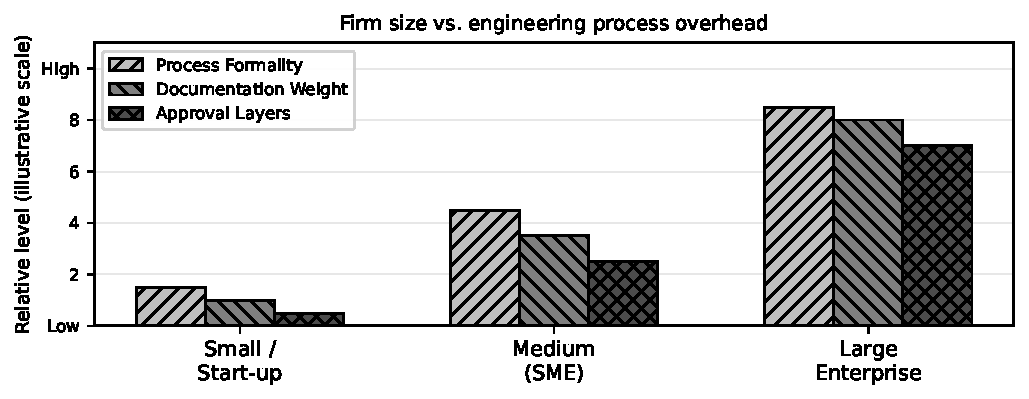
\includegraphics[width=0.85\textwidth]{images/fig_03_firm_spectrum.pdf}
  \caption{Firm-size spectrum: process formality, documentation weight,
           and approval layers all increase substantially from small
           start-ups to large enterprises.
           The prototype development approach must match the firm context.}
  \label{fig:ch1-firmspectrum}
\end{figure}

\textbf{Small firms and start-ups}\index{start-up} (under $\approx$20
people) move fast and tolerate ambiguity.
A single engineer may own the entire design.
Documentation is minimal---often just enough to reproduce the build.
The prototype is frequently made by the same people who conceived it.
Speed matters more than process.
The risk is that institutional knowledge lives in people's heads and
disappears when they leave.

\textbf{Medium firms (SMEs)}\index{SME} (20--500 people) have begun to
institutionalise.
There are defined roles, some formal review gates, and more documentation
requirements.
A design change needs sign-off from more than one person.
The prototype team is likely distinct from the product team, so
documentation quality directly affects the handoff.

\textbf{Large enterprises}\index{large enterprise} (500+ people) operate
under heavy process---ISO standards, stage-gate reviews, change control
boards, formal test plans, and full configuration management.
A prototype at a large firm may require months of internal approval before
the first component is ordered.
Documentation must be complete, traceable, and auditable.

None of these contexts is inherently better.
A start-up that adopts enterprise process collapses under bureaucratic
overhead.
A large firm that abandons process loses traceability and produces
unrepeatable results.
Your job is to recognise the context you are in and calibrate your
documentation effort accordingly.

\paragraph{In Practice.}
A three-person IoT start-up builds a temperature monitoring module in four
weeks: breadboard, firmware, cloud logging, mobile app.
The ``documentation'' is a shared folder with photos and a text file.
Two years later, the same company has grown to forty people.
A new hire tries to reproduce the original circuit for a customer
request.
The photos are there; the design rationale is not.
It takes three weeks to reverse-engineer the component selection.
The original four weeks of work left a four-week debt that compounded
with every new hire.

% ──────────────────────────────────────────────────────────
\section{Science for Profit: Cost, Time, and Volume}
\label{sec:ch1-science-for-profit}
% ──────────────────────────────────────────────────────────

Engineering work is not science for its own sake---it is science directed
at creating value.
This does not diminish the intellectual content; it sharpens the
questions.
In a commercial context, every technical decision carries an economic
consequence, and the three most important constraints are \textbf{cost},
\textbf{time}, and \textbf{volume}.
\index{cost}\index{time}\index{production volume}

\textbf{Cost} constrains what you can build and at what margin.
A solution that is technically elegant but costs twice the target
variable cost is not a viable product.

\textbf{Time} constrains competitive advantage.
A prototype finished six months late may miss a market window entirely.
Time is the one resource you cannot recover.

\textbf{Volume} determines the economic structure.
At low volumes, fixed costs (tooling, engineering, certification) dominate
the per-unit cost.
At high volumes, variable costs dominate.
Chapter~10 develops this model formally; here, it is enough to recognise
that the prototype's per-unit cost---often assembled by hand from
individual components---tells you nothing about what the product will cost
at 1,000 units.

A critical professional skill is the ability to interpret a negative
economic finding correctly.
Suppose your prototype proves that the design works but the cost analysis
shows that no viable margin exists at any realistic production volume.
This is not failure---it is the most valuable result the prototype could
have produced.
You have saved the firm the cost of a full product development effort on
an unviable design.
Document the finding clearly, state the assumptions, and let the
engineering team decide whether to pivot or stop.
A prototype that says ``no'' is doing exactly what a prototype is for.

% ──────────────────────────────────────────────────────────
\section{How a Prototype Becomes Revenue}
\label{sec:ch1-revenue-models}
% ──────────────────────────────────────────────────────────

Validating a prototype is not the end of the story.
The business question that drives the prototype is always, ultimately:
how does this create value that someone will pay for?
Figure~\ref{fig:ch1-bizmodels} maps the major revenue models available
once a prototype has been validated.
\index{revenue model}\index{business model}

\begin{figure}[htbp]
  \centering
  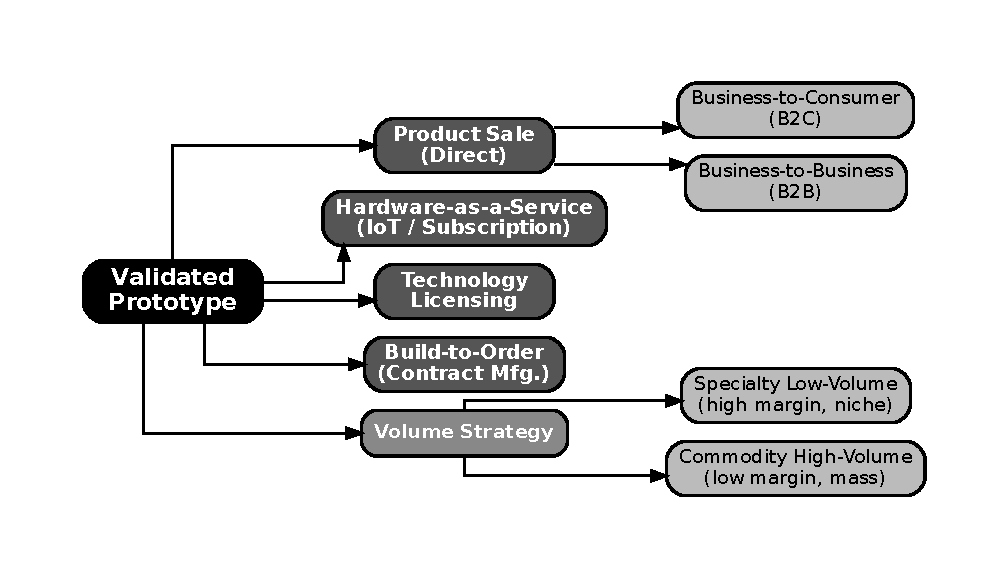
\includegraphics[width=0.85\textwidth]{images/fig_04_business_models.pdf}
  \caption{Revenue models reachable from a validated prototype.
           The choice of model shapes what the prototype must prove and
           what the product development effort must deliver.}
  \label{fig:ch1-bizmodels}
\end{figure}

\textbf{Product sale (direct).}
\index{product sale}
The most familiar model: manufacture a unit, sell it for more than it
costs to make and sell.
The two dominant sub-types differ in who the customer is.
In a \textbf{business-to-consumer (B2C)}\index{B2C} model, you sell to
individuals; volume is potentially high but margins are typically lower
and customer acquisition is expensive.
In a \textbf{business-to-business (B2B)}\index{B2B} model, you sell to
companies; volumes are lower but unit prices and margins are generally
higher, and relationships carry more weight than brand.

\textbf{Hardware-as-a-Service (HaaS / IoT subscription).}
\index{hardware-as-a-service}
The customer pays an upfront hardware fee and a recurring subscription
for connectivity, data processing, and support.
The prototype must prove both the hardware function \emph{and} the
cloud-connectivity architecture.
This model creates recurring revenue and customer lock-in but requires
ongoing operational cost for the cloud backend.
It is common for IoT devices that produce data the customer values
continuously.

\textbf{Technology licensing.}
\index{licensing}
The firm does not manufacture; it licenses the design, firmware, or
algorithm to other manufacturers.
The prototype proves that the intellectual property is real and valuable.
Licensing requires strong IP documentation and often patents.
Beyond licensing, intellectual property ownership is a business-model consideration for every revenue model --- Chapter~15 covers the practical IP obligations a technician must understand.

\textbf{Build-to-order (contract manufacturing).}
\index{build-to-order}
The firm builds custom units against specific customer purchase orders.
Volume is low per customer; the customer drives the specification.
Margins can be high because the customer is paying for customisation.
The prototype is typically a demonstration to win the contract.

\textbf{Volume strategy: specialty vs.\ commodity.}
\index{specialty low-volume}\index{commodity high-volume}
Within product sale, the firm chooses where on the volume spectrum to
compete.
\textbf{Specialty low-volume} production targets niche markets with high
unit prices and high margins; low volume means less pressure on
tooling costs but fewer units over which to amortise fixed costs.
\textbf{Commodity high-volume} production targets large markets with low
unit prices and thin margins; every cent of variable cost matters, and
design-for-manufacture is mandatory from the first design decision.

The choice of revenue model is made before the prototype is designed,
not after.
It shapes what the prototype must prove, what fidelity is needed, and
what documentation must be produced.
A HaaS prototype that lacks a working cloud connection has not answered
the central business question.
A licensing prototype with no IP documentation has nothing to license.

% ──────────────────────────────────────────────────────────
\section*{Worked Example: The Sorting Subsystem Business Case}
\label{sec:ch1-worked-example}
% ──────────────────────────────────────────────────────────

Throughout this book, every chapter works through the same running
example: a \textbf{connected IoT robotic sorting subsystem}---a
sensor-guided actuator that classifies items on a bench conveyor,
diverts them to the correct output lane, reports status over a network,
and is designed as a module within a larger automation product.
\index{running example}

\textbf{Firm context.}
The team is a twelve-person engineering start-up that has identified
a market in light-industrial sorting for food processing and
pharmaceutical packaging.
The firm is too small for enterprise process but large enough to have
separate engineering and operations functions.
Documentation weight is medium: enough to enable reproduction by
another team member, not enough to require formal configuration management.

\textbf{Business model.}
The chosen model is \textbf{Hardware-as-a-Service}: customers purchase
the sorter module at a hardware price and pay an annual subscription for
cloud-hosted analytics, remote monitoring, and firmware updates.
This model requires the prototype to prove two things: (1) the mechanical
and electronic sorter works reliably, and (2) the cloud connectivity
architecture is sound and can sustain the required data throughput.

\textbf{What the prototype must answer.}
The central question is: \emph{Can a sub-\$500 CAD bill-of-materials
sorter module achieve $\ge$95\% sort accuracy at 6~items/min while
maintaining a reliable MQTT connection over a standard Wi-Fi network?}
If yes, the hardware is viable and the HaaS model can proceed.
If no, the firm needs to know whether the failure is in the mechanical
design, the sensing, the firmware, or the network layer---so the
portfolio must be structured to show that.

\textbf{Margin calculation.}
Suppose the firm targets a hardware unit price of
$p = \$1{,}200$~CAD and estimates the variable cost of a production
unit (materials + direct labour at volume) at
$c_{\text{var}} = \$480$~CAD.
(These are early estimates; Chapter~10 will refine them using the
full cost model.)

The unit margin is:
\begin{equation}
  m = p - c_{\text{var}} = \$1{,}200 - \$480 = \$720 \text{ CAD/unit.}
  \label{eq:ch1-margin}
\end{equation}

The gross margin fraction is:
\begin{equation}
  \text{GM} = \frac{p - c_{\text{var}}}{p}
            = \frac{\$720}{\$1{,}200}
            = 0.60 \quad (60\%).
  \label{eq:ch1-gm}
\end{equation}

A 60\% hardware gross margin is strong for an electromechanical module.
It must, however, sustain both the hardware warranty cost and the ongoing
cost of the cloud subscription infrastructure.
Chapter~10 will introduce the full unit-cost model,
$C_{\text{unit}}(N) = C_{\text{fixed}}/N + c_{\text{var}}$,
which shows how the fixed non-recurring costs (tooling, firmware
development, certification) dilute this margin at low production volumes.

\textbf{Project context brief (your first portfolio artifact).}
\begin{itemize}
  \item \emph{Project:} IoT robotic sorting subsystem module.
  \item \emph{Business model:} Hardware-as-a-Service; hardware sale +
        annual cloud subscription.
  \item \emph{Firm context:} 12-person engineering start-up; medium
        documentation weight.
  \item \emph{Business question the prototype must answer:}
        Can the module achieve $\ge$95\% sort accuracy at 6~items/min
        with a reliable cloud connection, at a BOM cost below \$500~CAD?
\end{itemize}

\subsection*{Try It Yourself}

A micro-robotics start-up is developing a vision-guided pick-and-place module.
They plan to sell it directly to electronics assembly firms (B2B product sale).
Their target unit price is $p = \$950$~CAD and their estimated variable cost is
$c_{\text{var}} = \$285$~CAD.

\begin{enumerate}
  \item Compute the unit margin $m = p - c_{\text{var}}$.
  \item Compute the gross margin fraction $\text{GM} = (p - c_{\text{var}})/p$
        and express it as a percentage.
  \item Using Figure~\ref{fig:ch1-bizmodels}, identify which revenue model applies
        and state one thing the prototype must prove to make that model viable.
\end{enumerate}

\noindent(Answers not provided — work through the arithmetic before moving on.)

% ──────────────────────────────────────────────────────────
\paragraph{Common Pitfalls.}
% ──────────────────────────────────────────────────────────

\textbf{Technically impressive $\neq$ good prototype.}
A prototype that demonstrates six different features but answers none of
the business questions clearly is not a good prototype.
Novelty and complexity are not success criteria.
The success criterion is: \emph{did you answer the question?}

\textbf{"It works" $\neq$ "the business case is proven."}
A prototype that demonstrates function but carries a BOM cost of
\$1,400~CAD against a \$1,200 target price is not a viable product,
regardless of how well it works.
The economic analysis is not an afterthought---it is half of the
prototype's output.

\textbf{Underrating the technician's judgment.}
Engineers rely on your observation that the actuator is running hotter
than expected, that the network connection drops in the presence of the
motor drive, or that a component you received does not match the
datasheet.
These observations, documented and communicated promptly, are the inputs
that prevent costly mistakes.
Do not wait to be asked.

\textbf{Reading a negative economic finding as failure.}
If the cost analysis shows that the HaaS model is not viable at any
realistic volume, that result should be reported clearly, not buried or
explained away.
The firm can decide to pivot---to a different revenue model, a
different component set, or a different market.
It cannot decide anything if the analysis is suppressed.

\section*{Review Questions}
\addcontentsline{toc}{section}{Review Questions}

\begin{enumerate}

  \item \textbf{(Conceptual)} A product must satisfy five properties that a
  prototype does not. List all five and write one sentence explaining what each
  requires in practice.

  \item \textbf{(Conceptual)} The chapter states that ``a prototype that returns a
  negative economic result is not a failure.''
  Explain this claim in your own words. What should the team do with the finding,
  and why is suppressing it dangerous?

  \item \textbf{(Applied --- calculation)} A start-up prices a wireless sensor node
  at $p = \$340$~CAD and initially estimates $c_{\text{var}} = \$136$~CAD.
  \begin{enumerate}
    \item Compute $m$ and $\text{GM}$\%.
    \item After a detailed BOM review, the true variable cost is
          $c_{\text{var}} = \$204$~CAD. Recompute $m$ and $\text{GM}$\%.
    \item By how many percentage points did the gross margin change?
          Comment on whether the product remains financially attractive.
  \end{enumerate}

  \item \textbf{(Applied --- classification)} A company has developed a
  machine-learning algorithm that identifies crop disease from smartphone photos.
  They plan to license it to agricultural equipment manufacturers.
  Using Figure~\ref{fig:ch1-bizmodels} and the definitions in §\ref{sec:ch1-revenue-models},
  identify the revenue model and state two things the prototype must demonstrate
  to support that model.

  \item \textbf{(Applied --- multi-step)} A proof-of-concept prototype costs
  \$2{,}400~CAD to build.  The team estimates that the eventual product will sell
  at $p = \$600$~CAD with $c_{\text{var}} = \$180$~CAD.
  \begin{enumerate}
    \item Compute $m$ and $\text{GM}$\%.
    \item The \$2{,}400 build cost is \emph{not} $c_{\text{var}}$.
          Name the cost category it belongs to, and explain why it does not
          appear in the margin formula at this stage.
          (\emph{Hint: Chapter~10 will introduce the full cost model.})
  \end{enumerate}

\end{enumerate}

% ──────────────────────────────────────────────────────────
\section*{End-of-Chapter Artifact: Project Context Brief}
\label{sec:ch1-artifact}
% ──────────────────────────────────────────────────────────

By the end of Week~1, you will produce a one-page \textbf{project context
brief}\index{project context brief} for your own project.
It is the first document in your portfolio and frames everything that
follows.
It must contain:

\begin{enumerate}
  \item A description of the project (one paragraph, no jargon).
  \item The chosen business model, with a one-sentence justification.
  \item The firm context (size, documentation standard, your role).
  \item The single business question the prototype must help answer.
  \item A preliminary margin estimate: state $p$, $c_{\text{var}}$,
        compute $m$ and GM\%, and note the assumptions behind
        $c_{\text{var}}$.
\end{enumerate}

Keep the brief to one page.
Its purpose is not comprehensiveness but clarity: after reading it, a
second team member should be able to say whether the project is
technically and commercially plausible at a first glance.

% ──────────────────────────────────────────────────────────
\section*{Summary}
\label{sec:ch1-summary}
% ──────────────────────────────────────────────────────────

Project~I delivers two things: a proof-of-concept prototype and the
portfolio that documents how you built and tested it.
The prototype's job is to answer one specific technical and business
question---not to be a miniature product.
Between Project~I and Project~II lies a deliberate gap: manufacturability,
reliability, cost at volume, certification, and supportability must all
be designed into the product in Project~II, using the prototype's answers
as a foundation.

As a technician, you own the build, the test, the documentation, and the
procurement.
Your hands-on judgment is the most direct input the engineering team has
to reality.

Firms handle prototypes differently depending on their size: start-ups
move fast with minimal process; enterprises move carefully with heavy
documentation.
Calibrate your effort to the context.

The economic constraints---cost, time, and volume---are design variables,
not external obstacles.
A prototype that returns a negative economic result is not a failure; it
is evidence.
The revenue model chosen before the prototype is built shapes everything:
what the prototype must prove, what fidelity is required, and what
documentation must be produced.

\medskip

\noindent\textbf{Up next:} Chapter~2 establishes the formal product development process --- the Cooper Stage-Gate model and Kano analysis --- that gives every subsequent chapter its professional context. You will see where this course and Project~II sit within that model, and how Kano analysis determines what the prototype must prove.
